\section{Project summary}

In this project we will attempt to answer the research questions shown in figure \ref{fig:Research_Questions}.
\begin{figure}[H]
    \centering
    \fbox{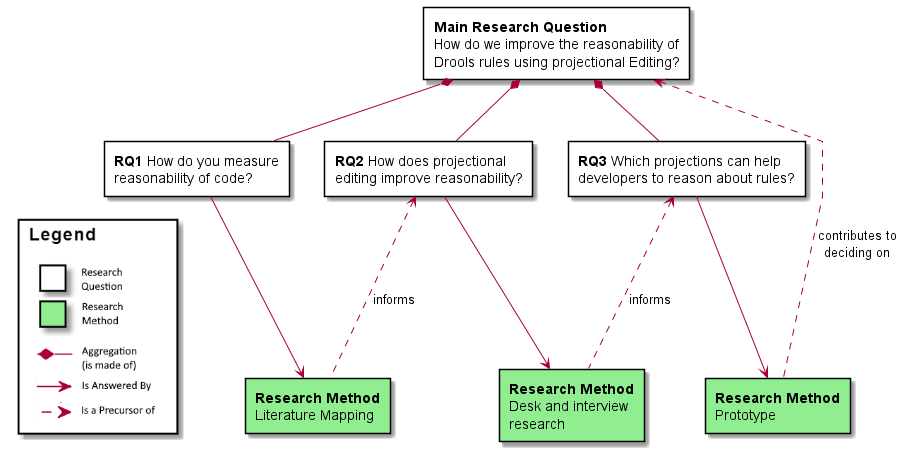
\includegraphics[width=0.95\textwidth]{images/ResearchQuestion_Legend.png}}
    \caption{Research Questions and Methods}
    \label{fig:Research_Questions}
\end{figure}


Drools\cite{browne2009jboss} is an open-source production rule system for complex event processing, using an implementation of the Rete algorithm\cite{forgy1989rete}.
It has a Domain Specific Language (DSL), in which rules are described.
These are stored in Drools (.drl) files. 
Reasoning over a small number of rules is already surprisingly hard.
Our host organization has many rules and, thus, reasoning about them is particularly challenging.
This master's project will attempt to improve how one can reason about Drools rules.

Editing in language workbenches has two predominant editing forms - free-form text editing and projectional editing\cite{erdweg2013state}.
Free-form text editing is the more popular of these two.
Projectional editing is a method of bypassing the need for a parser and programming directly into projections of the Abstract Syntax Tree.

We will create such an editor for the Drools DSL using a language workbench capable of creating projectional editors.  
On top of this newly modelled DSL, we will create new and different projections of the code for the purpose of increasing the reasonability of the code. 
To be clear, by reasonability we mean having the ability to reason.

For this project we will use the open-source language workbench Meta Programming System (MPS) from JetBrains\cite{MPS_ProductPage}.
MPS is built around the projectional editing paradigm.
There is no existing implementation of the Drools language in MPS.

Although Drools is nearly 20 years old and has wide use, it does not have strong IDE support.
One artefact of this master's project will be a prototype projectional editor, that will give much stronger editor support in IntelliJ, currently the most used Java IDE\cite{Java_usage_report}.
